\documentclass[12pt]{article}
\usepackage{graphicx}
\usepackage{listings}
\usepackage{hyperref}
\usepackage[utf8]{inputenc}
\usepackage{amsmath}
\usepackage{amsfonts}
\usepackage{amssymb}
\usepackage{datetime}
\usepackage{float}
\usepackage[export]{adjustbox}
\usepackage{longtable}
\usepackage{geometry}
\usepackage{algpseudocode}
\usepackage{algorithm}
\geometry{a4paper, margin=1in}

\makeatletter
%algorithmic font size
\renewcommand{\ALG@beginalgorithmic}{\tiny}
\makeatother

\title{Comparative Analysis of Physical and Virtual Spring Reverb Technologies}
\author{
    Shaojun Chen(s736chen), Jackson He(z262he), Honglin Cao(h45cao) \\
}

\newdate{date}{05}{04}{2024}
\date{\displaydate{date}}
\begin{document}

\maketitle

\begin{abstract}
This project aims to explore the auditory and technical differences between a physical spring reverb pedal, a virtual simulation of spring reverb implemented as a script and some commercially available spring reverb plugin. By designing, building, and testing a physical spring reverb pedal, and concurrently developing a digital emulation using Octave, we seek to understand how each medium affects audio signal processing and listener perception. The project will culminate in a comparative analysis based on technical measurements and subjective listening tests.
\end{abstract}

\tableofcontents
\newpage

\section{Introduction and Design}
\subsection{Background of spring reverb}

Reverb, short for reverberation, is a fundamental audio effect that adds depth, spaciousness, and realism to sound recordings and live performances. It occurs when sound waves reflect off surfaces in an environment and then reach our ears, creating a complex blend of delayed and attenuated sound reflections. This phenomenon is what gives a sense of space, whether it's the natural reverberation in a cathedral, the intimate ambiance of a small room, or the ethereal quality of a dreamy musical track. Musicians, audio engineers, and producers often use various reverb techniques and equipment to enhance their audio recordings and achieve desired sonic characteristics.

Spring reverb was first introduced in the early 1930s by Laurens Hammond. Best known for the Hammond organ, was the first device to use a spring reverb unit. However, it was not until the 1960s that it became widely popular, thanks to its incorporation into guitar amplifiers.

Spring reverb have been a cornerstone in audio effects processing, providing distinctive reverberation effects that are difficult to replicate accurately with digital technology. The physical properties of springs contribute unique characteristics to the audio signal, which digital simulations strive to emulate.
Spring reverb is known for its unique, sometimes ``boingy'' or ``twangy'' quality, and it has been used in various musical genres, from surf rock to dub reggae. It offers a different sonic character compared to other reverb types like plate, hall, or room reverbs, making it a favourite among musicians and producers looking for a vintage or distinctive sound.


\subsection{Design of physical spring reverb unit}

For this project, we firstly googled and find some photos of reverb tanks used in traditional guitar amplifiers. Most of the modern designs has the spring suspended in the gap of a transducer, and a transducer push and pulling on the spring causing them to vibrate at the same frequency as the audio signal.\footnote{``Mod Reverb Tanks - Spring Reverbs Explained.'' Mod Reverb Tanks - Spring Reverbs Explained | Mod Electronics. n.d. Web. 05 Apr. 2024. } And the receiving side was identical to the inputting side, with the vibration of the spring transformed into electronic signal by the transducer.

\begin{figure*}[h]
	\center
	\includegraphics[width=0.3\linewidth]{photos/small_tank_out_detail.png}
	\caption{A closer look of a commercial reverb tanks}
\end{figure*}

However, this type of spring reverb utilized custom-made transducer, which meant copying this design would be impossible for us, as we lacked the knowledge and tools to fabricate a custom transducer from scratch. So we went with an easier route: connecting the spring directly to a speaker, and let it pushing and pulling directly on the spring create longitudinal wave into the spring. This design might change the characteristics of the resulting signal, as the inputting wave onto the spring is longitudinal rather than transversal, and this could be an interesting comparison to look into.

For the speaker, we come across some very nice looking surface transducer, which is meant to transfer vibrations to large surfaces to create audible sounds, and they are essentially just conventional speakers with the paper cone replaced by a piece of metal.

For the receiving side, we decided to go with conventional guitar piezo under-saddle pickup to save some time on designing and manufacturing, plus we can use existing guitar amp or sound interface to get a cleaner sound from it rather than use some cheap amplifier board for a transducer.

As for the springs, since it's the core of any spring reverbs, we were unable to find any specifications for it used in commercial spring reverbs units. So we could only source some stainless steel pulling springs from ali-express and ems-store from Engineering 3 with various diameter and length, and we settled with one of them that have the lowest pulling force and largest diameter to hopefully achieving a longer decay rate, so the reverb effects could be more obvious.

\subsection{Design of software spring reverb}

Initially we planned to develop a virtual version of a spring reverb as a VST audio plugin. However, we encountered some complexity issues of the algorithms, as we discovered the convolution processing is not possible to implement into a real-time plugin without dedicated hardwares, and all such plugins were heavily simplified and very difficult to understand. Therefore, we decided to use Octave for asynchronous audio processing. To achieve this, we carefully read 2 papers and summarized the principles of physical spring reverb into devising a relatively simple algorithm so we could finish in the timeframe of this term, since the primary goal was to model the physical spring with algorithms rather than making it pleasing to listen. 

We referenced two pieces of articles and designed a simplified spring reverb model based on the content of ``Efficient Dispersion Generation Structures for Spring Reverb Emulation'' by Julian D. Parker. This paper focused primarily on enhancing the efficiency of digital simulation for spring reverb, as well as how to reduce the computational cost of digital reverb. The paper mentioned that traditional digital spring reverb's reliance on all-pass filters and delays to achieve dispersion effects, which was also an important reference part of our design. The main portion of the article discussed how to improve the computational efficiency and simulation fidelity of digital reverb by splitting different components based on traditional digital reverb. However, our goal was to simulate spring reverb using software, so we didn't need to consider efficiency issues a lot. Therefore, we only referenced the first half of the article.

From our experience in making the physical spring reverb, we knew that when sound passes through a spring, it experienced certain frequency losses due to the spring's inherent frequency, making the sound warm due to the reduction of high frequencies after passing through the spring. Therefore, we designed a low-pass filter to reduce the high frequencies of the signal. Moreover, a portion of the signal bounced back and sent to the output after the sound passes through the spring again, which was implemented with a delay line to simulate this physical property of the spring.

The fundamental framework included digital audio processing in Octave, filter design and simulation of the propagation and the decay of waves inside the spring. The filter was to simulate the dispersion effect and frequency decay of the spring. The feedback delay network with decay was to simulate multiple reflections and propagation of signals in the spring. Finally, the wet signal will be mixed with the original signal and sent to the output. 

\begin{figure*}[h]
	\center
	\includegraphics[width=0.6\linewidth]{photos/reverb.drawio.png}
\end{figure*}

In the above figure, we splited the input into two copies. One for the dry mix, and the another one for the spring algorithm to precess. Finally, we mixed them and wrote it as the output file. For the spring signal, the copy of the input first goes through a filter. Then, the processed signal was sent to the output, and a portion of the decay signal is sent back through the delay line into the filter again. The signal undergoes multiple overlaps, presenting a delayed effect. By controlling the delay time and adjusting the filter parameters, we achieve a simple simulation of the spring reverb effect.

%%%%%%%
\subsubsection{Reverb model}

The model we purposed had the following two main components:
\begin{itemize}
	\item \textbf{Delay Network}: A set of delay buffers is used to simulate the multiple back-and-forth travels of sound within a spring. Each buffer contains the feedback signal for a specific time delay, which can easily record the delayed signal in different round trips. For each loop or round trip, the feedback level of the sound will decrease. Thus, we design a decay rate to adjust the feedback level after each sound reflection, simulating the energy loss as the sound propagates through the spring material.
	
	\item \textbf{Filter}: Due to the intrinsic frequency and material characteristics of the spring, sound signals passing through the spring will result in the decay of a certain frequency. Our filter, based on the spring's intrinsic frequency, makes corresponding adjustments to specific frequency bands of the sound, particularly the high frequencies. This approach renders the high frequency of the spring reverb softer. 
	
\end{itemize}

And the following parameters we could change:

\begin{itemize}
	\item \textbf{Feedback level \& Decay rate}:  These parameters together determine the duration and decay speed of the reverb. Higher feedback gain and lower decay rates result in a longer-lasting reverb effect, while the opposite leads to a quicker dissipation of reverb. To simulate the spring reverb. Adjusting these parameters can simulate springs of different material properties. We can modify the ``\texttt{initial\_delay\_ms}'' and ``\texttt{decay\_rate}'' in the code to adjust the feedback level and decay rate.
	
	\item \textbf{Delay Time \& Echo times}: The delay time determines the time in milliseconds that the signal takes to propagate within the spring. The echo times determine the number of round trips a signal can travel. The longer delays can simulate longer springs, creating a richer reverb effect. The delay time is always set to be 20ms to 50ms. We can modify the ``\texttt{initial\_delay\_me}'' and ``\texttt{num\_echoes}'' in the code to adjust the delay time and echo times.
	
	\item \textbf{Mix Rate}: The mix ratio of the reverberated signal and the original signal. The big mix rate will produce more spring reverb signals, while the opposite leads to a less reverb sound. We can modify the ``\texttt{mix\_rate}'' in the code to adjust the mix rate.

	\item \textbf{Filter Frequency}: Adjusting the cut-off frequency of the filter can simulate the impact of spring physical characteristics on the sound's frequency response. A lower cut-off frequency simulates greater decay of high-frequency components, producing a warmer, more natural reverb effect.
	
\end{itemize}

%%%%%%%%%%%%%%%%%%%%%%%%
\newpage
\section{Implementation}

In this section of our report, we delve into the practical aspects of bringing our conceptual designs to life. This chapter is dedicated to providing a comprehensive overview of our journey from conceptualization to realization, including both our hardware and software development processes for the spring reverb project, as well as .

\subsection{Testing clip}



\subsection{Hardware spring reverb}

\begin{longtable}{| p{.21\textwidth} | p{.79\textwidth} |} 
\hline
\textbf{Photo} & \textbf{Description} \\
\hline

\includegraphics[width=0.2\textwidth,valign=c]{photos/IMG_7909.jpg} & 
purchased surface transducer, driver board for the transducer, guitar piezo pickup, 6.5mm audio jack and several metal springs. \\ 
\hline

\includegraphics[width=0.2\textwidth,,valign=c]{photos/IMG_8080.jpg} & 
Used a power supply board and a bread board from my Arduino kit, prepare to solder the wires. \\ 
\hline

\includegraphics[width=0.2\textwidth,,valign=c]{photos/IMG_8082.jpg} & 
Soldered the pin to the transducer driver board. \\ 
\hline

\includegraphics[width=0.2\textwidth,,valign=c]{photos/IMG_8084.jpg} & 
The power supply board needs 9V battery, trying to use my Raspberry PI Zero 2W to power the driver board instead. Used multimeter to determine the 5V and GND. \\ 
\hline

\includegraphics[width=0.2\textwidth,,valign=c]{photos/IMG_8085.jpg} & 
Soldered the surface transducer to a GPIO pin for easier connection later. \\ 
\hline

\includegraphics[width=0.2\textwidth,,valign=c]{photos/IMG_8086.jpg} & 
Connected both the driver board and the transducer itself to the bread board with Arduino cables. \\ 
\hline

\includegraphics[width=0.2\textwidth,,valign=c]{photos/IMG_8095.jpg} & 
The 6.5 jack I purchased is stereo, even though we are only doing a mono output, but I soldered 3 wires to it. \\ 
\hline

\includegraphics[width=0.2\textwidth,,valign=c]{photos/IMG_8096.jpg} & 
Soldered piezo pickup to 2 wires as well, i want to try to drive the piezo pickup with the transducer driver board. \\ 
\hline

\includegraphics[width=0.2\textwidth,,valign=c]{photos/IMG_8097.jpg} & 
 Redo the GPIO pins only for 5V and GND so I can mount driver boards directly onto the bread board, and soldered the 6.5 Jack to the input and output of driver boards respectively, also soldered the piezo pickup to the input of one of the driver board.\\ 
\hline

\includegraphics[width=0.066\textwidth,,valign=c]{photos/IMG_8745.jpg} 
\includegraphics[width=0.066\textwidth,,valign=c]{photos/IMG_8746.jpg} 
\includegraphics[width=0.066\textwidth,,valign=c]{photos/IMG_8748.jpg} & 
Measuring the dimension of the surface transducer for designing housing for the spring reverb. \\ 
\hline

\includegraphics[width=0.2\textwidth,,valign=c]{photos/IMG_8749.jpg} & 
 Design and FDM 3D printed a hook that i will glue to the surface tranducer to hold the spring. \\ 
\hline

\includegraphics[width=0.2\textwidth,,valign=c]{photos/IMG_8767.jpg} & 
 Glued the hook to the surface transducer.\\ 
\hline

\includegraphics[width=0.066\textwidth,,valign=c]{photos/IMG_8770.jpg}
\includegraphics[width=0.066\textwidth,,valign=c]{photos/IMG_8771.jpg}
\includegraphics[width=0.066\textwidth,,valign=c]{photos/IMG_8772.jpg} & 
Doing some measurement on the piezo pickup for designing housing for spring reverb. \\ 
\hline

\includegraphics[width=0.1\textwidth,,valign=c]{photos/IMG_8773.jpg}
\includegraphics[width=0.1\textwidth,,valign=c]{photos/IMG_8774.jpg} & 
Designed the housing for spring reverb in Fusion 360, output to PrusSlicer for printing on SLA resin printer. \\ 
\hline

\includegraphics[width=0.2\textwidth,,valign=c]{photos/IMG_8776.jpg} & 
 Also designed a seperated version to glue on together later, just to make sure at least one version will be available.\\ 
\hline

\includegraphics[width=0.2\textwidth,,valign=c]{photos/IMG_8779.jpg} & 
SLA resin print finished \\ 
\hline

\includegraphics[width=0.2\textwidth,,valign=c]{photos/IMG_8783.jpg} & 
Post processing done \\ 
\hline

\includegraphics[width=0.2\textwidth,,valign=c]{photos/IMG_8784.jpg} & 
Mount components to the housing, dimension seems correct. \\ 
\hline

\includegraphics[width=0.2\textwidth,,valign=c]{photos/IMG_9382.jpg} & 
To prevent vibration of the surface transducer, applied automotive foam tape to the housing printed previously for gluing up. \\ 
\hline

\includegraphics[width=0.2\textwidth,,valign=c]{photos/IMG_9383.jpg} & 
Applied foam tape to the two sides, so when bounding the 3 piece together the vibration wouldn't affect the piezo pickup system. \\ 
\hline

\includegraphics[width=0.2\textwidth,,valign=c]{photos/IMG_9384.jpg} & 
Connect the 3 piece using duct tape, so the joint (foam tape) is flexible and able to absorb vibrations.\\ 
\hline

\includegraphics[width=0.2\textwidth,,valign=c]{photos/IMG_9385.jpg} & 
Installed all the components to the housing. \\ 
\hline

\includegraphics[width=0.2\textwidth,,valign=c]{photos/IMG_9593.jpg} & 
The amplifier for the surface transducer is broken somewhere, it's no longer functioning. Will use my bookshelf speaker amp to drive the surface transducer, it should be even better than the original amplifier I built for the surface transducer.\\ 
\hline

\includegraphics[width=0.2\textwidth,,valign=c]{photos/IMG_9594.jpg} & 
Take the speaker cable connector from my DIY bookshelf speaker \\ 
\hline

\includegraphics[width=0.2\textwidth,,valign=c]{photos/IMG_9596.jpg} & 
Connected the cable connector to the surface transducer. \\ 
\hline

\includegraphics[width=0.2\textwidth,,valign=c]{photos/IMG_9597.jpg} & 
The amp works really well (it even has EQ adjustments), and the damping foam tape works as well, only around 20\% of the surface transducer's vibration is able to reach the plate housing the piezo pickup. Now it shouldn't affecting the piezo pickup anymore. \\ 
\hline

\includegraphics[width=0.2\textwidth,,valign=c]{photos/IMG_9603.jpg} & 
Some testing shows the surface transducer is moving inside the hole holding it creating some squeaking sound. Applied some UV curing resin to the surface transducer and using UV curing station for SLA printer to cure the resin. \\ 
\hline

\includegraphics[width=0.2\textwidth,,valign=c]{photos/IMG_9604.jpg} & 
Now the surface transducer is permanently mounted to the housing plate.  \\ 
\hline

\includegraphics[width=0.2\textwidth,,valign=c]{photos/IMG_9605.jpg} & 
Final recording setup completed. \\ 
\hline

\end{longtable}

\newpage
\subsubsection{Recording setup}

The driving of surface transducer was accomplished by connected an iPhone to the amplifier via BlueTooth, which connected to the surface transducer through two GPIO extension cable. The piezoelectric pickup which attached to the spring, was connected to my sound interface \textbf{Apollo Solo}, which in turn was connected to a laptop running\textbf{Logic Pro}. Then, we played the test clip from the iPhone and started recording in Logic Pro.

Due to the piezo pickup being designed for guitar use, its sensitivity was insufficient for capturing vibrations from the spring. Therefore, we had to increase the gain for the piezo pickup to +52 dB on the sound interface (hardware gain) to capture any sound, which also amplified the noise. Subsequently, we have to use the \textbf{X-noise} plugin from Waves to mitigate these noises, otherwise we cannot compare the spectrum later on. Even though applying the noise reduction plugin resulting in reduced detail.

\begin{figure*}[h]
\center
	\includegraphics[width=0.5\linewidth]{photos/xnoise.jpg}
	\caption{Using plugin to cancel the noises}
\end{figure*}

\subsubsection{Future developments}

During the recording process, we found that when the amplifier for the surface transducer was turned too high, it would resulting in the spring touching itself (too much vibration on the spring), which will create some rather loud artifact and disrupt the actual signal. So, we have to lower the gain of the amplifier, which resulted in needing to +52 dB on the receiving end while recording, which resulted in an extensive amount of noise.

\begin{figure*}[h] 
	\center 
	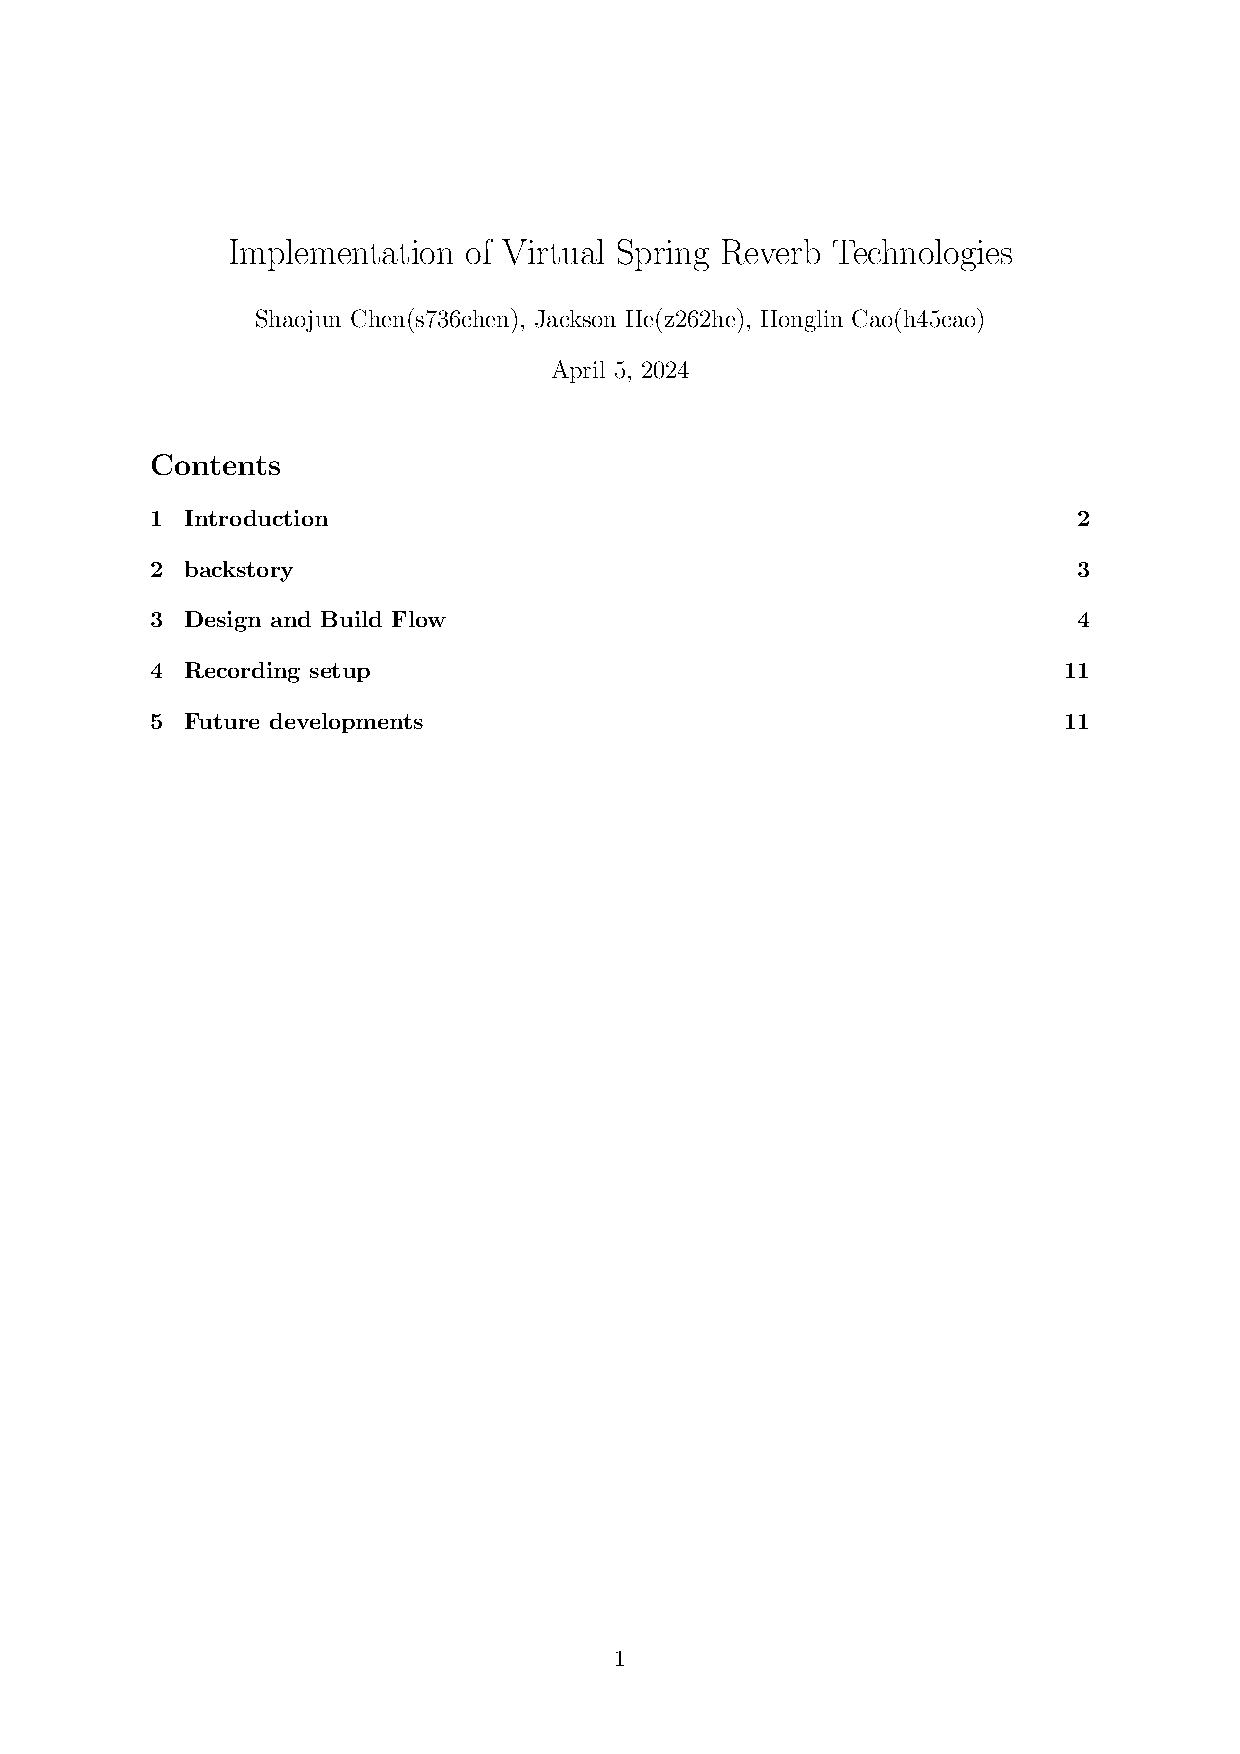
\includegraphics[width=0.5\linewidth]{photos/spring.jpg} 
	\caption{Spring used in my reverb tank} 
\end{figure*} 

Similar issue wasn't found on the commercial spring reverb tanks, presumably due to the fact that our implementation created longitudinal wave rather than transversal comparing to the commercial solutions; And it may also due to the fact that the spring we used has too many coil numbers, so it's very easy for the coils to touch each other when the amplitude was large. To mitigate this, we could find some extension spring that has the same diameter for the wire but way less coil number. However, the one we got was the only one left in the E3 mechanical store. So finding a suitable spring was quite hard and couldn't be completed in time for this project. 

Secondly, even though the spring was not suitable, the piezo pickup was definitely not sensitive enough for capturing vibrations of the tiny spring. To improve this, we will need to find some other piezo pickup systems that are not designed for under-saddle usage for guitars, rather for sticking on the surface of an instrument to capture the vibrations, which should be more sensitive. Also, this couldn't be accomplished due to the time constraints of this project.

Lastly, the use of foam tape with duct tape seems quite effective for stopping the vibration, but after sitting there for a few days, it showed some level of deformation under the tension of the spring. So, some other mechanism not involving duct tape and foam tape was needed. we had originally decided to use some spring to suspend the surface transducer somewhere, but the supporting structure for this seemed not possible to be 3D printed. Also, to design and actually create such structure was also impossible to accomplish due to the time constraints of this project.

\begin{figure*}[h] 
	\center 
	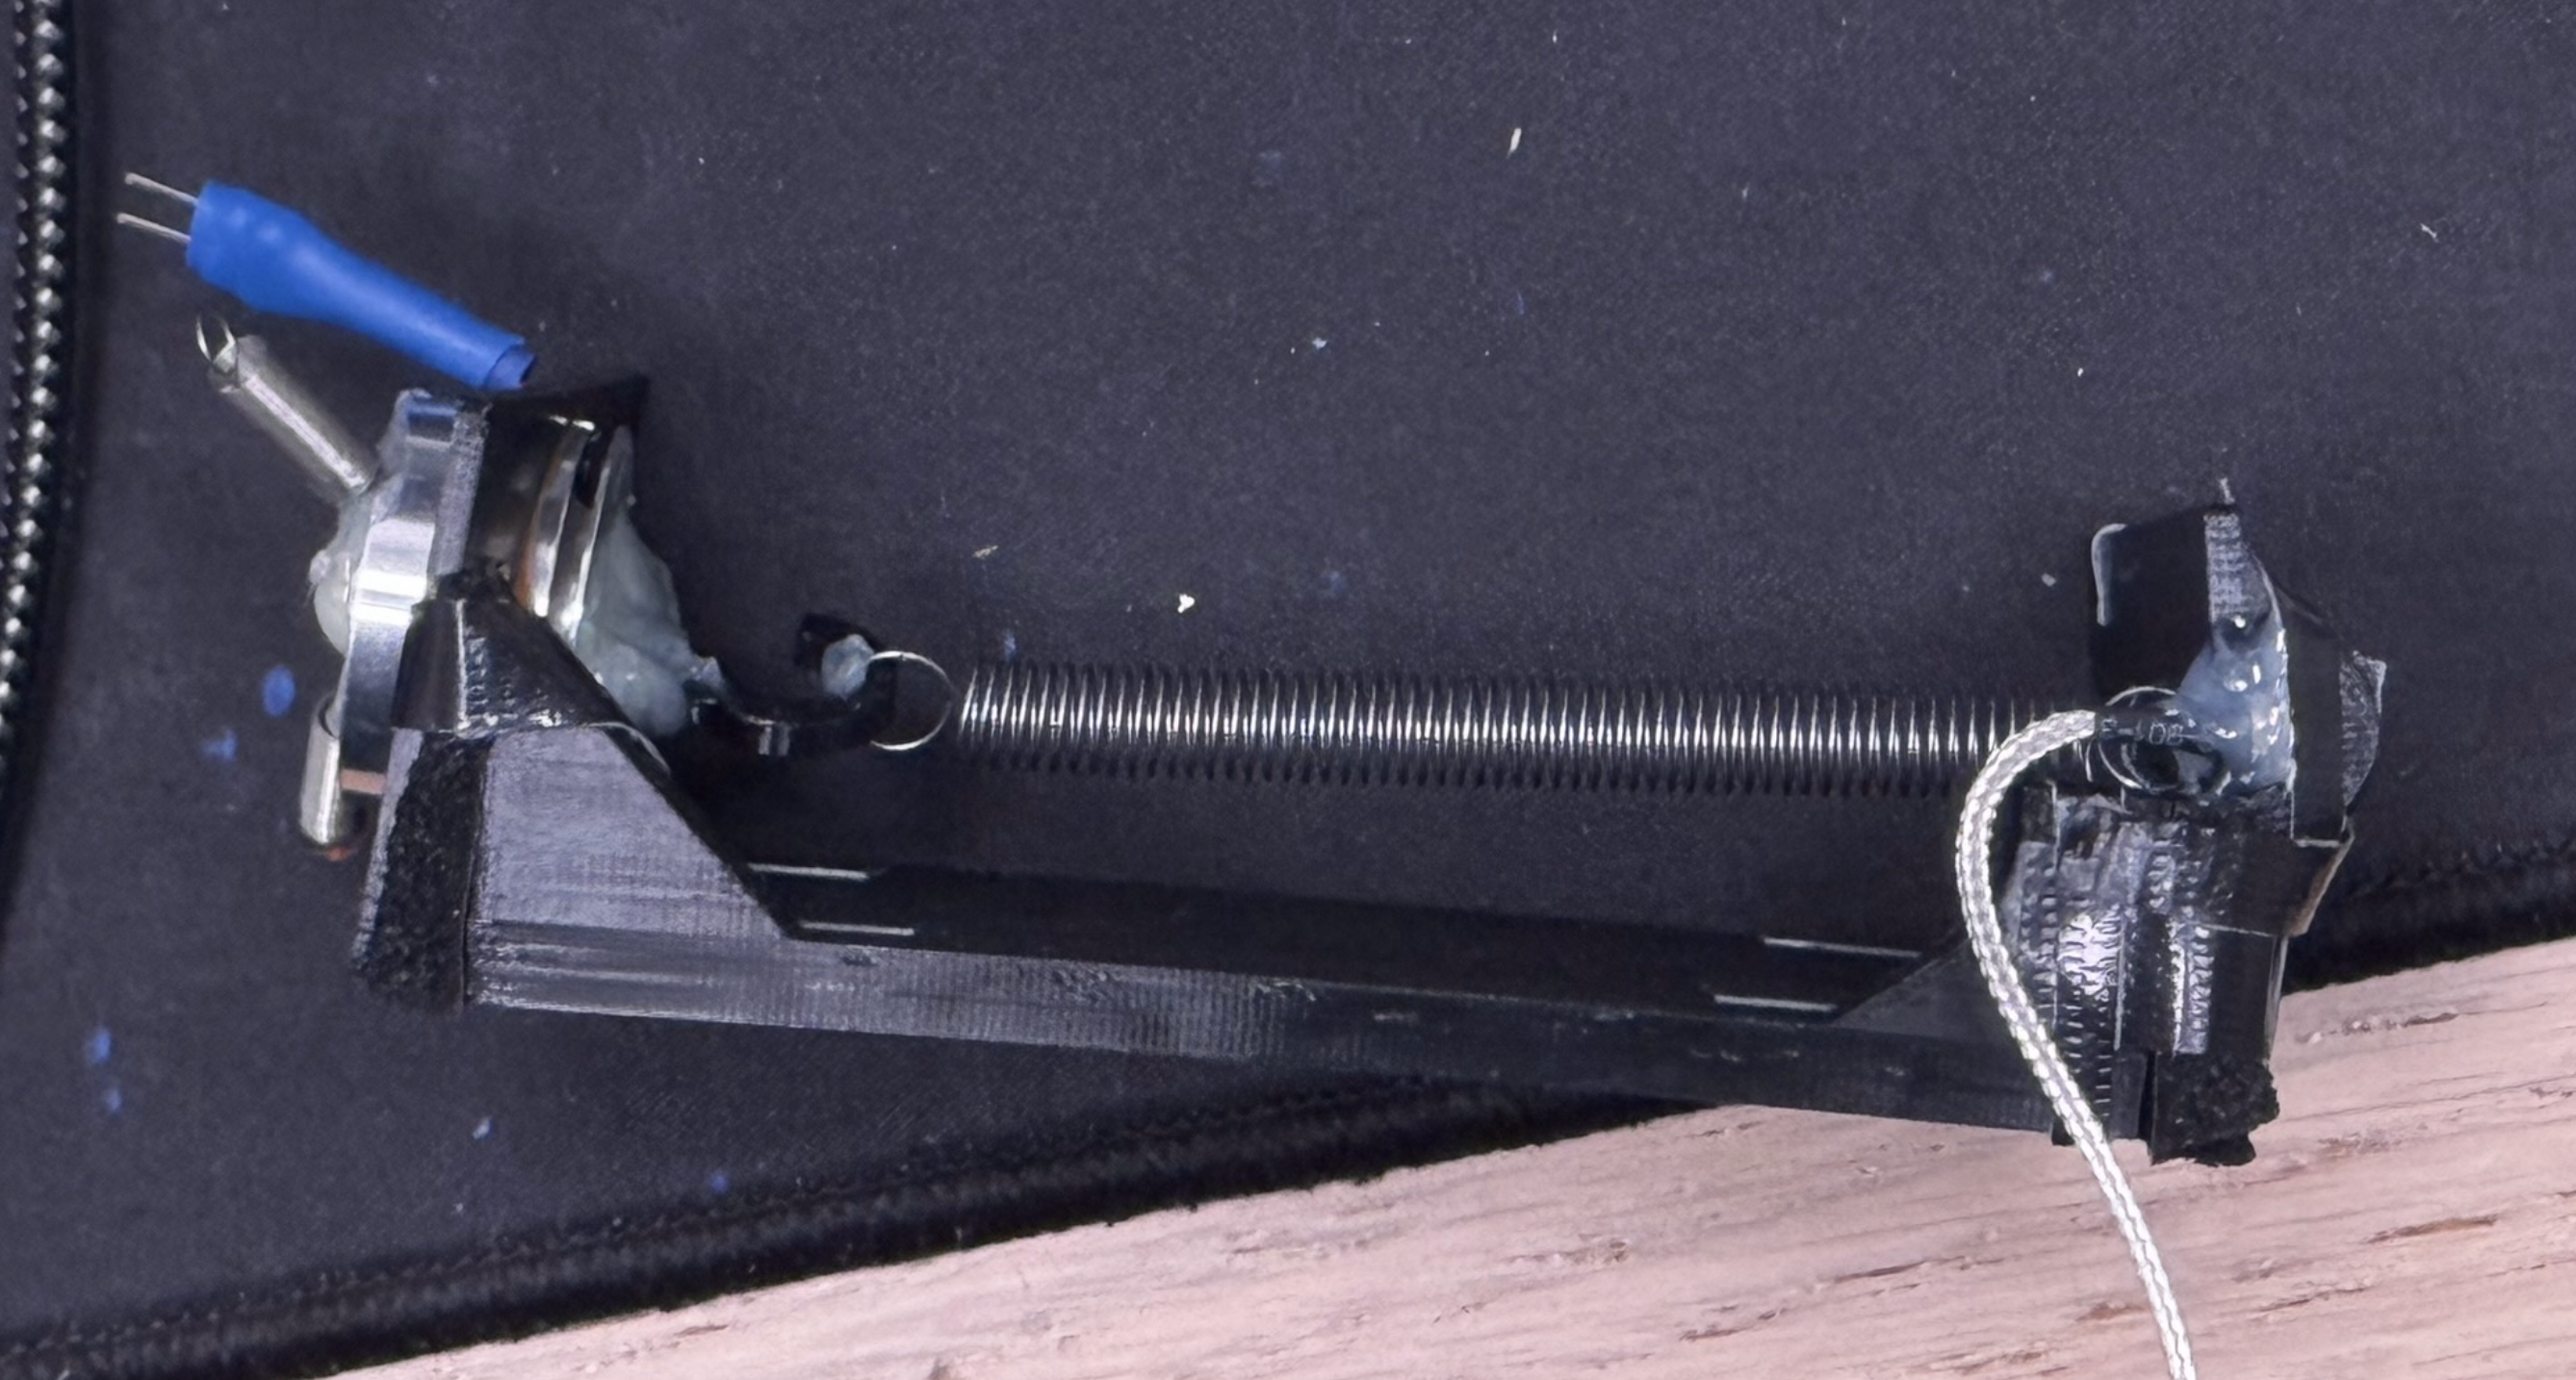
\includegraphics[width=0.5\linewidth]{photos/deformation.jpg} 
	\caption{Housing is no longer straight under the tension of the spring} 
\end{figure*} 
%%%%%

\newpage
\subsection{Software spring reverb}
The implementation of the software Spring Reverb was in the Octave script ``\texttt{spring\_reverb.m}''. This function will take an input WAV file and produce a processed output file in mono signal. 

We can modify the file name in line 40: \texttt{\footnotesize [input\_signal, fs] = audioread(`test\_melody.wav')} to modify the input file. Then, in last line 93: \texttt{\footnotesize audiowrite('output\_melody.wav', reverbed\_signal, fs)} you can modify the output file name.  Also, to achieve a different spring effect, we can modify the parameters in the code as described in section 1.3.1.

To implement the filter, we used a Gaussian filter centred around the natural frequency of the spring. We applied FFT and IFFT to obtain the filtered signal. The \texttt{spring\_filter} function was used to filter the input signal, simulating the effect of the spring's natural frequency on the sound. While implementing the delay network, we used a loop and buffer to record the decay signal to add the reverb effects to the output signal. We recorded the delay buffer and calculated the superposition of multiple echoes. The intensity of each was decreased according to the feedback gain and decay rate. 

Finally, the reverb signal and the original signal were mixed following a set ratio (60\% wet in our code\footnote{\scriptsize If we set the mix ratio to 100\% wet, all the outputs will sounds just like a delay effect due to our implementation. Plus, our physical reverb implementation's housing also directly transmitted portion of the dry signal to the piezoelectric pickup. And 60\% was decided because it produced the most pleasing tone on our testing clip.}) and written as the new output signal. 

\begin{algorithm}
\caption{Spring Reverb Simulation Pseudocode}

\
\begin{algorithmic}[1]
\State Load the signal processing package.

\
\Procedure{spring\_filter}{$input\_signal, fs, f\_natural$}
    \State Perform FFT on $input\_signal$.
    \State Generate a Gaussian filter centered around $f\_natural$ in the frequency domain.
    \State Apply the generated filter to the FFT results.
    \State Perform IFFT to obtain the filtered signal.
    \State \textbf{return} $filtered\_input\_signal$
\EndProcedure

\
\State Read WAV file into $input\_signal$.
\State Convert $input\_signal$ to mono if it is in stereo.
\State Initialize simulation parameters:
\begin{itemize}
    \item $N$: Length of $input\_signal$
    \item $output\_signal$: An array of zeros with length $N$
    \item $initial\_delay\_ms$: The initial delay length in milliseconds
    \item $num\_echoes$: The total number of echoes
    \item $feedback\_initial\_level$: The initial feedback gain level
    \item $mix\_rate$: The mix ratio of the reverberated signal and the original signal
    \item $decay\_rate$: The decay rate after each reflection
    \item $spring\_natural\_freq$: The natural frequency of the spring
\end{itemize}

\
\State Initialize the delay buffer and calculate the delay sample length for each echo.

\
\State Preprocess $input\_signal$ with \Call{spring\_filter}{} function.

\
\For{each sample in $input\_signal$}
    \State Add the current sample to the delay buffer.
    \For{each echo}
        \State Calculate the echo sample using the delay buffer.
        \State Accumulate the echo samples.
    \EndFor
    \State Add the accumulated echo samples to $output\_signal$.
\EndFor

\
\State Mix the original signal with $output\_signal$ based on $mix\_rate$.
\State Normalize the mixed signal.
\State Write the normalized signal to 'output\_melody.wav'.
\end{algorithmic}
\end{algorithm}

\newpage
\subsubsection{Future developments}

Our current model incorporated a basic implementation of dispersion through delay line and filtering. Moving forward, we will explore more advanced physical modelling techniques to simulate the dispersion effects. For instance, we can further calibrate the phase of the audio signal to achieve the effect of dispersion, and incorporate the impulse response (IR) of an actual spring to achieve a more complex and authentic reverb effect.

Although we omitted the issue of computational efficiency this time to simplify the process, we could investigate into turning the algorithm we proposed into a real-time software in the future, which enable it as a tool we could use for live performance and real-time recording applications. This involves refactoring our code architecture, improving overall execution efficiency and considering the delay in the output of the effect. We will reference the sections on algorithm efficiency in the paper ``Efficient Dispersion Generation Structures for Spring Reverb Emulation'' for improvements.

%%%%%%%%%%%%%%%%%%%%%%

\newpage
\section{Evaluation and Comparison}

\newpage
\section{Conclusion}


\end{document}
